\subsubsection*{Training Insights}
EfficientNet did not produce useful predictions on any of the ten training runs. Even the best model struggled to estimate galaxy cluster masses precisely. Especially with lower mass clusters, the model was not able to get close to the true values as seen in \autoref{fig:best_perf_EffB7_a} and \ref{fig:best_perf_EffB7_b}. The predictions look somewhat similar to the VGG predictions, in that they are cut off at a certain value, in this case at around $\log{(M_{500}^{\text{true}}/M_{\odot})} \sim 13.5$.

\subsubsection*{Best Performing Model}
The best performing EfficientNetB7 model suffered from the same problems as the other EfficientNetB7 models trained. Its predictions are cut of at the lower end and on the training predictions, two lines are visible where the model seemed to prefer two mass areas for its predictions.

\begin{figure}[H]
\centering
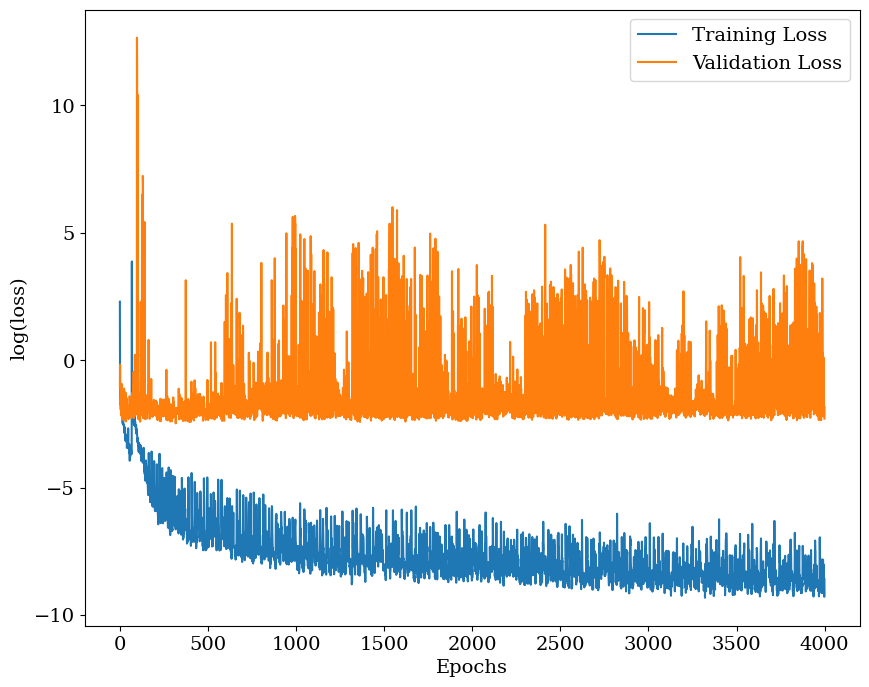
\includegraphics[width=.667\textwidth]{images/Chapter4/EffB7/eff_history.png}
\caption{Training history of the best performing EfficientNetB7 model. The spiking validation loss indicates that the training did not produce good results.} 
\label{fig:EffB7_best_history}
\end{figure}
While the training loss kept decreasing, the validation loss was spiking at many epochs during training. The model seemed to have problems finding anything useful to improve validation accuracy. As seen in the model's predictions, the model was not even able to make predictions in the correct mass range.


\begin{figure}[H]
\centering
\begin{subfigure}{.46\textwidth}
  \centering
  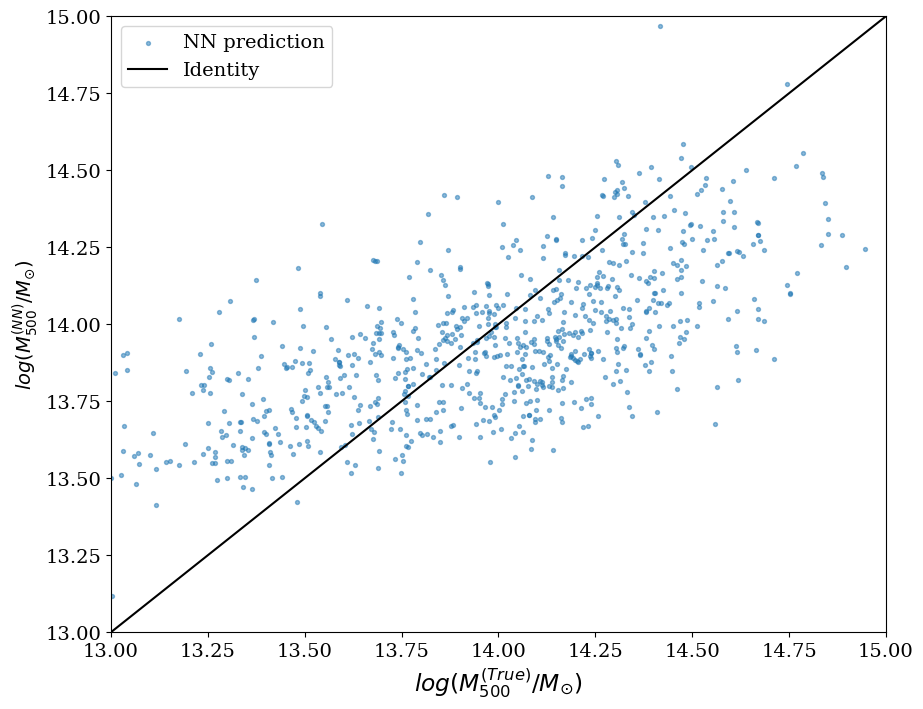
\includegraphics[width=\linewidth]{images/Chapter4/EffB7/eff_test.png}
  \caption{Model predictions on the test set.}
  \label{fig:best_perf_EffB7_a}
\end{subfigure}%
\hspace{.6em}
\begin{subfigure}{.46\textwidth}
  \centering
  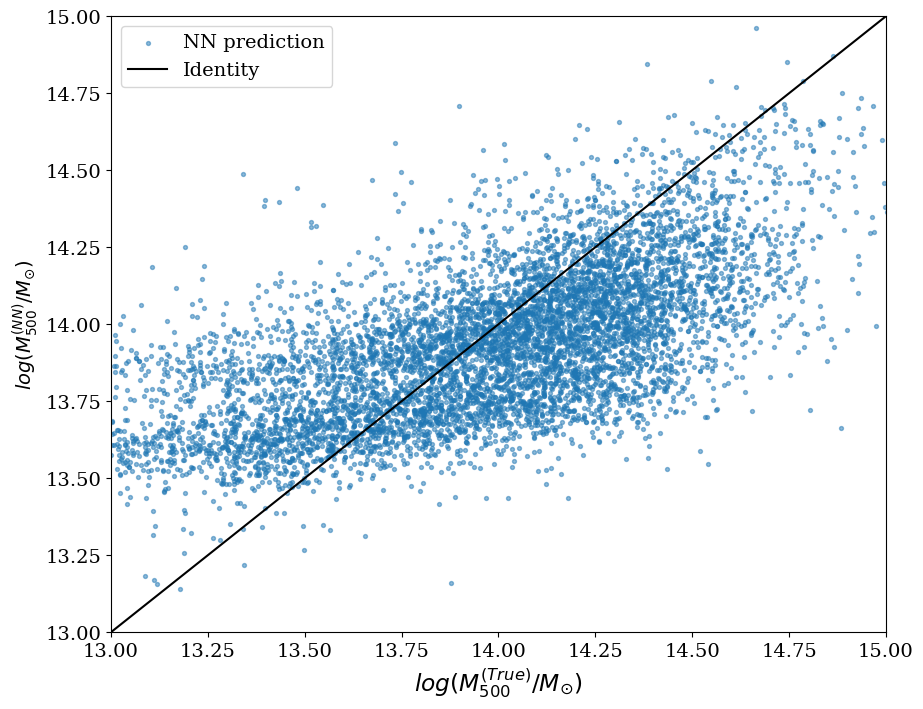
\includegraphics[width=\linewidth]{images/Chapter4/EffB7/eff_train.png}
  \caption{Model predictions on the training set.}
  \label{fig:best_perf_EffB7_b}
\end{subfigure}
\begin{subfigure}{.46\textwidth}
  \centering
  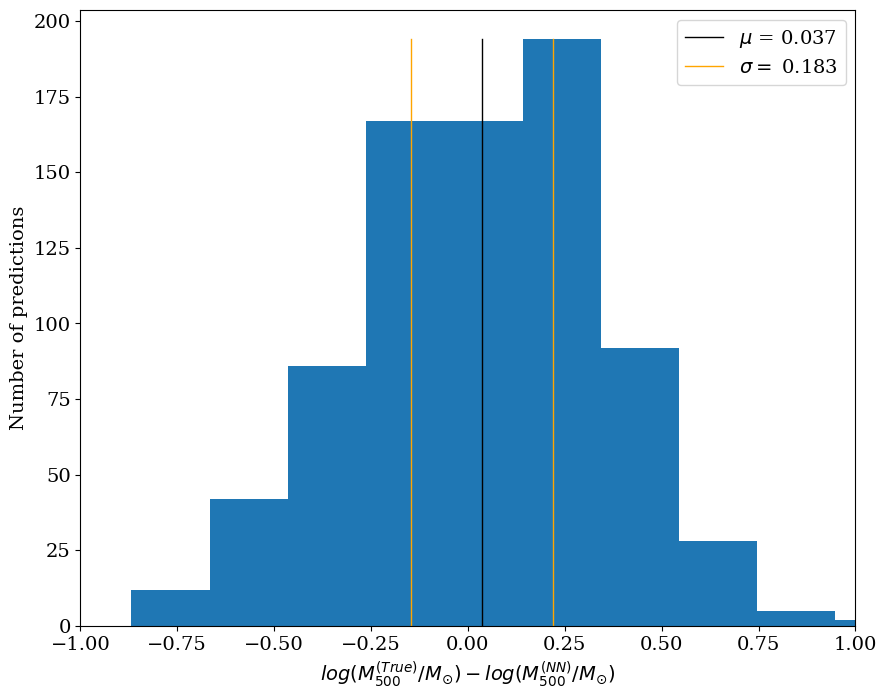
\includegraphics[width=\linewidth]{images/Chapter4/EffB7/eff_test_hist.png}
  \caption{Histogram of model predictions on the test set.}
  \label{fig:best_perf_EffB7_c}
\end{subfigure}%
\hspace{.6em}
\begin{subfigure}{.46\textwidth}
  \centering
  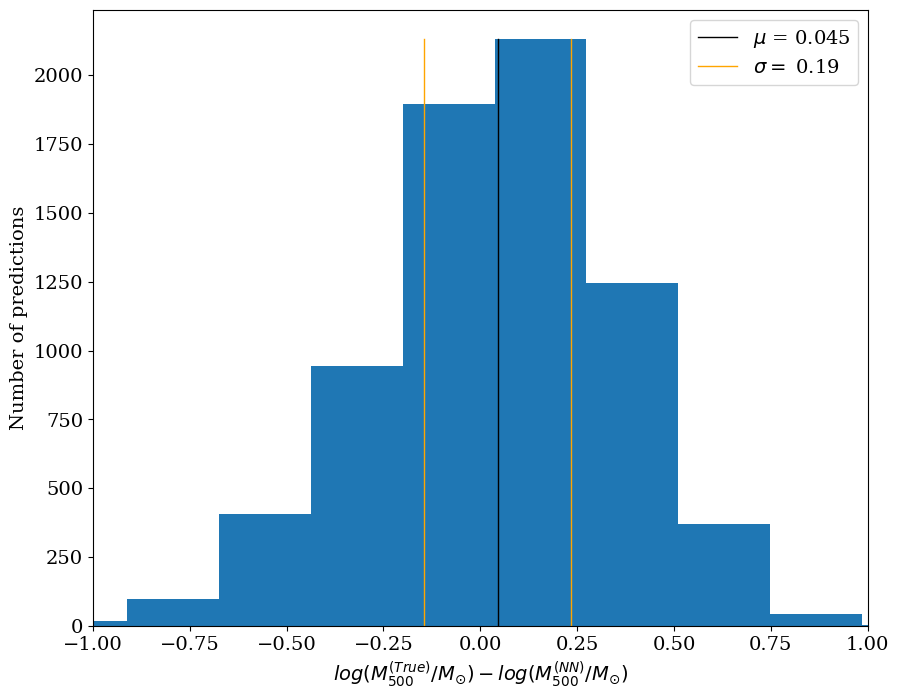
\includegraphics[width=\linewidth]{images/Chapter4/EffB7/eff_train_hist.png}
  \caption{Histogram of model predictions on the training set.}
  \label{fig:best_perf_EffB7_d}
\end{subfigure}
\caption{Results of the best EfficientNetB7 model.} 
\label{fig:best_perf_EffB7}
\end{figure}

Because of these problems, the overall prediction accuracy is not close to the best ResNets or the basic CNN with a $\sigma$ of $0.183$ on the test set. Astonishingly, despite the low training loss, the predictions on the training set are not overfitted or anywhere near the identity (see \autoref{fig:best_perf_EffB7_b}). Considering the enormous training time for this model and its lacking accuracy, I would not recommend further investigation of this model for galaxy cluster mass estimation.